\documentclass{article}

% taken from doron for the bib
\usepackage{amsmath,amsthm,mathtools,amsfonts,graphicx,epsfig}
\usepackage[justification=justified,singlelinecheck=false,nooneline,font={footnotesize}]{caption}
%\usepackage[font={footnotesize }]{subcaption}
\usepackage[sort&compress]{natbib}
\usepackage{geometry}
\usepackage{epstopdf}  %for use with pdflatex
\usepackage[usenames,dvipsnames]{color}
\usepackage{colortbl}
\def\bibfont{\footnotesize}
\usepackage{float}

\usepackage{amssymb}
\usepackage{graphicx}
\usepackage{algorithm}
\usepackage{algorithmicx}
\usepackage[noend]{algpseudocode}
\usepackage{algpseudocode}
\usepackage{multicol}
\usepackage{color}
\definecolor{lightyellow}{RGB}{255,255,160}
\definecolor{lightred}{RGB}{255,119,119}
\usepackage{caption}
\usepackage{subfigure}
%\usepackage{scicite}
\DeclareMathOperator*{\argmax}{arg\,max}
\graphicspath{C:/Users/Yair/Dropbox/Thesis/figures/}

\title{Co-Occurring Clustering}
\author{}
\date{\today}
\begin{document}
\maketitle

\section{Introduction}
Data clustering is a useful tool for all kind of applications,
Unsupervised clustering has a wide spread of solution and algorithms which are based on the definition of a cluster and some parameters(known analogy is the difference between k-means and spectral clustering ).
Clusters are easier to distinguish when they have a sufficient slackness margin (i.e., they are separable and do not overlap). When dealing with noised data clustering becomes a problem and traditional method fail to distinguish between clusters.
Most traditional clustering methods deal the data as if it was chosen i.i.d from an unknown distribution. For some cases this is not the case, we will show an unsupervised clustering method- \textbf{Co-Occurring Clustering}  for images, that only assumes the data is not iid by using some labeling statistics.

To test our clustering we will use a version of Non-Local Means \cite{NL-means}, That is averaging each pixel with it's in-cluster neighbors.
To illustrate that good clustering =  good denoising, an example is given in figure \ref{fig:ORACLE clustering}
Image denoising based on such noisy clustering will result poor results.

\begin{figure}[!hb]
	\subfigure [Noisy input]
	{\includegraphics[width=9.2em,height=9.2em]{{"C:/Users/Yair/Dropbox/Thesis/figures/Mtex Noisy"}.jpg}}
	\quad
	\subfigure [Basic Denoising]{\includegraphics[width=10em,height=10em]{{"C:/Users/Yair/Dropbox/Thesis/figures/Mtex Dnoised"}.jpg}}
	\quad
	\subfigure [ORACLE denoising]{\includegraphics[width=10em,height=10em]{{"C:/Users/Yair/Dropbox/Thesis/figures/Mtex Dnoised ORACLE"}.jpg}}
	\caption{(a) Noisy input with additive Gaussian noise $ \sigma=40 $ (b) denoising the image with cluster formed from the noisy data (c) denoising the image with ORACLE labeling. i.e., simple clustering done on a zero noise image.}\label{fig:ORACLE clustering}
\end{figure}

\subsection{General idea}
We think of basic clustering done on a zero noise image as the ground truth of labeling. as shown in figure [\ref{fig:ORACLE clustering}] this labeling gives good denoising results. Another feature of the ground truth clustering ia a sparse Co-Occurrence matrix (will be discussed).
Our idea is to capture the Co-Occurrence properties when clustering a noisy image as shown in figure \ref{fig:sparsity}.
\begin{figure}
	\includegraphics[width=0.8\textwidth]{{"CC Sparsity"}.jpg}
	\caption{Co-Occurrence matrix. left image is for ground truth labeling for 'barbara', center image is for noisy clustering. Right image is the Co-Occurrence for the noisy image after applying Co-Occurring Clustering}\label{fig:sparsity}
\end{figure}

 By capturing the Co-Occurrence structure we form clusters that their data points may be less dense, but that create a spatial 'repetitive' texture in the image. Another way to look at it, instead of trying to find the latent ground truth labeling, we try converging into a sparse Co-Occurrence matrix.
 
 This repetitive property can be shown in the multi-texture image from figure \ref{fig:ORACLE clustering}, where each texture is divided into several clusters separately. Labeling the entire image based on those clusters (actually, cluster centers) form a distinctive block structure Co-Occurrence, shown in figure [\ref{fig:block CC}], implying that each texture is formed by a small amount of clusters.
\begin{figure}
	\includegraphics[width=0.6\linewidth]{{"C:/Users/Yair/Dropbox/Thesis/figures/CC of MultiTexture using ORACLE"}.jpg}
	\caption{In a multi texture image, we learned 50 clusters centers for each texture separately, we used those 250 ($ 50X5~ $textures) centers to form a simple nearest neighbor clustering. We can see a block structure in the Co-Occurrence matrix which can be understood that each texture is defined mainly by its original centers}\label{fig:block CC}
\end{figure}
\section{Notations}
Given an image I with $ n $ pixels. We define a labeling function $ \widehat{L} $:
\begin{equation*}
\widehat{L}:(1,..,n)\rightarrow (1,..,K)
\end{equation*}
i.e., $ \widehat{L}_{(i)}=J \qquad\text{ states that: }pixel~i \in cluster~J $\footnote{we use small letters to denote a pixel and Large letters for cluster labels}

\subsection{Visual space}
The feature vector representing pixel $ i $ in visual space will be column stacking of the window patch of size $W_1\times W_1$ around it.
\begin{equation*}
W_{(i)}\in \mathbb{R}^{W_{1}^{2}}
\end{equation*}
Clustering the image in visual $ \mathbb{R}^{W_{1}^{2}} $ space, we denote cluster's $ J $
Center in visual space as:  $C_{J}=\dfrac{1}{|J|} \Sigma_{\widehat{L} (i)=J}~W_{(i)}$
i.e., the center of cluster $ J $ is the mean of all pixels that are labeled in the cluster ($i\in cluster~J$).

We will denote:
\begin{equation}
P_{i}(J) =\dfrac{1}{Z}exp^{(\dfrac{-dist(W_{(i)} ),C_J)}{\sigma_s〗^2})}〗\label{eq:pixelPr}
\end{equation} 
The probability that pixel i$\in cluster~J$,
where $ dist(\cdot,\cdot) $ is the Euclidean distance.(sometimes we will refer as P[i,J] or $ \Pr\{i,J\} $ for matrix notation)

We will also use:
\begin{equation}
P(J)=\frac {|J\vert}{n}
\end{equation} 
For the non local label probability.
\subsection{Labels histogram space}
For this space representation, first we will look at the image $ L $ that instead of intensity, each pixel value is its cluster label, given by $\hat L$\footnote{Labels is categorical data with no respect to size $ J>K $}.

Each pixel in $ L $ will then be characterized by its label values histogram in a $W_2\times W_2$ window around it (not containing the center pixel).\\
e.g. 
\begin{multicols}{5}
	\begin{tabular}{|c|c|c|}\hline
		1&5&1\\	\hline
		5&\colorbox{lightred}{3}&5\\ \hline
		9&8&9\\ \hline
	\end{tabular}
	
	\begin{flushright}
		H*[i]=
	\end{flushright}	
	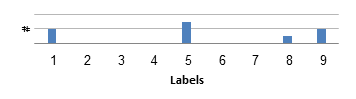
\includegraphics[width=2.2\linewidth]{histogram.png}
\end{multicols}
We denote $ H_{(i)} $ for the Histogram of pixel i in labels space, $ H_{(i)} $  is normalized to 1 (s.t. in the example $ H_{(i)} = \dfrac{\text{H*[i]}}{8}$ )\footnote{generally $\dfrac{\text{H*[i]}}{W_2^2-1}$ }\\
We will also use  $ H_{(i)}(J) $- the J coordinate in $ H_{(i)} \quad $. $ H_{(i)}(J)=\Pr \{\widehat{L}_{\mathcal{N}(i)}=J \} $
\begin{equation*}
H_{(i)}\in \mathbb{Z}^K 
\end{equation*}

\section{Co-Occurrence Clustering}
In order to get a dense cluster in visual spaces and simultaneously produce a sparse Co-Occurrence matrix, We want to minimize
\begin{align}
&\min\sum_i \psi_i +\lambda\sum_{i,m}\lVert\phi_{i,m}\rVert_0 \\
&\psi_i=dist(W_{(i)},C_{\widehat L_(i)}) \nonumber\\
&\phi_{i,m}=CC\nonumber
\end{align}
denoting $ CC $- the conditional probability Co-Occurrence matrix (other choices of $ \phi $ will be discussed).

\subsection{CC- Co-Occurrence Matrix}
A non formal definition for Co-Occurrence matrix, denoted as CC, is:
$ CC[J;K] =$ How much K co-occur around a know  $pixel~i\in cluster~J $
There are a few definitions for the CC matrix, we will use:
\begin{equation}
CC[J;K] =P(K|J) \tag{Conditional Co-Oc}
\end{equation}  

We use the labels statistics, to compute the conditional probability that two labels are adjacent.
\begin{equation}
P(K|J)= \frac{1}{|J|}\sum_{\forall i ~;\widehat{L}_{(i)}=J} P_{\mathcal{N}(i)}(K)
\label{eq:CoOc}
\end{equation}

where $ \mathcal{N}(i) $ is the neighbors of pixel i in $ W_2 $ window, and  $ |J|=|\{pixel\ i\in cluster\ J\}| $- the size of cluster J
In words we can say this is the probability to witness label K in $ W_2 $ window around a know pixel labeled J.\\
%A more formal definition should be:  $ P(K|J)=\dfrac{\sum_{i} P _j(K)}{P(J)} \ \ s.t. \begin{cases}
%&j \in {\mathcal{N}(i)}\\
%&\widehat{L}(i)=J
%\end{cases}  $ % I need to check the formolation Vs the code

We arrange $ P(K|J) $ to form a Co-Occurrence matrix, such that the element in the J-th row K-th column is: $ P(K|J) $
The Probability to witness Label $ K $ around a pixel known to be in $ J $ is: $ CC_J= P(K|J) $

The conditional probability Co-Occurrence matrix is not symmetric but can be normalized easily by choosing to use joint probability (This will be discussed later on).
\begin{equation}
P(K;J)=P(K|J)\cdot P(J) \label{eq:jointprob} \tag{Joint Probabilty Co-Oc}
\end{equation}

As showed in figure \ref{fig:sparsity}, labels Co-Occurrence matrix should be sparse\footnote{practically using $ \epsilon-norm $}, that is min $||CC||_0$. based on that assumption we will calculate an integrated probability function for each pixel $\Pr \{W_{(i)}\in cluster J\}$ and show that this regularization derives better assignment. 

\section{Co-Occurring clustering}
We would like to update equation \eqref{eq:pixelPr}- $ P_{i}(J) $ to relate to a data term- $ dist(W_{(i)}\, ,C_J) $ and regularization in the label space- $ \Vert
\phi\Vert_0 $.

\begin{equation}
\widetilde{P}_i(K) \leftarrow (1-\lambda) P_i(K) + \lambda\sum_{j\in N(i)}^{} P(K|\widehat{L}_{(j)}=J)\cdot P_{j}(J)
\end{equation}
We can think of it as a message passing from all of $\mathcal{N}(i)$-neighbors of pixel $ i $ combining with it's own belief. 

Based on the new posterior probability we would like to find the maximum likelihood estimator, so the $ \hat{L}_{ML} $ is given by:
\begin{equation}
\hat{L}=\argmax _{\hat{L}} \sum_{i}^{}P_i(\widehat{L}_{(i)})
\end{equation}

some remarks on the components of the update rule:
\begin{itemize}
	\item distance between the cluster center and $ W_(i) $- we would like a small distance to the cluster center.
	\item Co-occurrence matrix- each neighbor encourage his surrounding to resemble his Co-Oc.
	\item The neighbors probability $ H_(i) $- the more confidence your neighbor have, the more you should listen to him.
\end{itemize}


The procedure is given in algorithm \eqref{alg:Jointprobability} also shown in figure \ref{fig:Scheme}

\begin{algorithm}[!h] 
	\caption{Joint probability algorithm}\label{alg:Jointprobability}
	\begin{algorithmic}
		\State Initialize $\hat L$ using K-means on visual space
		\Loop
		\State update centers $C_{(J)}=\dfrac{1}{|J|} \sum_{\widehat{L}(i)=J}^{}P_{(i)}$
		\State calculate the matrices $ H_{(i)}(J),P_{(i)}(J) $
		\State Calculate the Co-Occurrence matrix  $ CC\gets INDICATOR\footnotemark\times H $
		\State hard threshold shrinkage $ CC(CC<Thr)\gets 0 $ \Comment{will be discussed}
		\State update: $ \widetilde{P}_i \leftarrow (1-\lambda)P_i + \lambda\sum_{j\in N(i)}^{} P(K|\hat{L}(j)=J)\cdot P_{j}(J) $
		%		$ L=(1-\lambda )\times S + \frac{\lambda }{W_2^2-1} \times H\times CC $
		\State $ \hat{L}(i)=\argmax _L(  P_i(L(i))  ) $
		\EndLoop
		\State \textbf{return} $\hat{L}$
		
	\end{algorithmic}
\end{algorithm}

\footnotetext{$\text{INDICATOR}[i,J]:=\begin{cases}
	1, &\text{ if }\hat L(i)=J\\
	0, &\text{ else}
	\end{cases} $}


\begin{figure}[ht]
	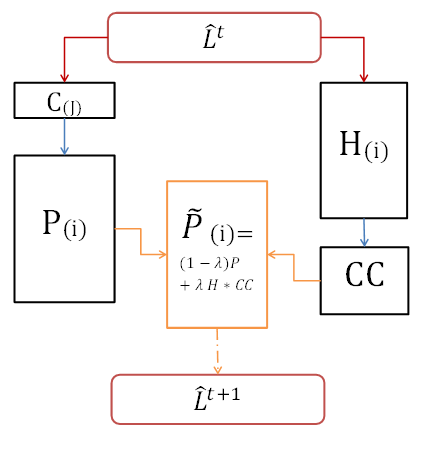
\includegraphics[scale=1.1]{Scheme1.png}
	\caption{Joint Probability Scheme}
	\label{fig:Scheme}
\end{figure}

\section{Others Co-Occurrences}

Our basic conditional Co-Occurrence is show at \eqref{eq:CoOc}, we showed an update rule for each pixel based on passing information from his surrounding.

An alternative method is calculating the Maximum Likelihood for the center pixel. maximizing The probability of the histogram given a certain label for the center pixel.
\begin{align}
\widehat{L}(i)&=\argmax_K \Pr~\{H_{(i)}|\widehat{L}(i)=K \}\\
&=\argmax_K\sum_{j\in\mathcal{N}(i)}^{} ~\sum_{M}^{} \Pr \{\widehat{L}(j)=M|\widehat{L}(i)=K \}\cdot P_j(M) \nonumber
\end{align}
This result a simple correlation distance between the neighborhood histogram $ H_{(i)} $ and the typical histogram for label K $ CC_k $.
As we mentioned before the CC matrix is not symmetric, hence, the two method of updating $ P_{i} $ will result different estimators.

In \eqref{eq:CoOc} we showed how to build the CC matrix from a hard assignment, one can also use soft assignment, which is:
\begin{equation}
P(k|J)=\frac{\sum_{i}H_{(i)}(K)\cdot P_i(J)}{\sum_{i} p_i(k)}
\end{equation} 

Another problem of the conditional Co-Occurrence is that label with low frequency will tend to disappear after some regularization. The reason is that we prefer to use a low amount of label to describe a texture and adding a low frequent label will drag a high penalty to this.

We can normalize our Co-Occurrence matrix to take into account the label frequency.
\begin{enumerate}
	\item joint probability of two label to co occur in the same window as showed in \eqref{eq:jointprob}.
	\item 'Mutual Information' Co-Occurrence which tries to capture how unique is to see two label co occur. 
	\begin{equation}
	M(K;J)=\dfrac{P(K|J)}{|K|} \tag{Mutual Co-Oc}
	\label{mutual CoOc}
	\end{equation} 
\end{enumerate}

Second can be thought as 'Mutual Information' variant which tells us how much the two label co occurring is unique.
\begin{equation}
M(K;J)=\dfrac{P(K|J)}{|K|}
\end{equation} 

\colorbox{lightyellow}{up to here...}


\bibliography{bibCoMeans}

\bibliographystyle{unsrt}
\section{testing}
$ \argmax $\\
\includegraphics[width=30em]{{"CC Sparsity"}.jpg}\\
\end{document}